\documentclass[11 pt]{article} % use larger type; default would be 10pt
\usepackage[utf8]{inputenc} % set input encoding (not needed with XeLaTeX)
\usepackage[T1]{fontenc}
\usepackage{authblk}

%%% BEGIN Article customizations

%%% PAGE LAYOUT
\usepackage{geometry} % to change the page dimensions
\geometry{a4paper} % or letterpaper (US) or a5paper or....
% \geometry{margin=1in} % for example, change the margins to 2 inches all round
\usepackage[parfill]{parskip} % Activate to begin paragraphs with an empty line rather than an indent

%%% FIGURES
\usepackage{graphicx} % support the \includegraphics command and options
\graphicspath{{../FIGURES/FIGURE_PDFS/}}

%%% PACKAGES
\usepackage{booktabs} % for much better looking tables
\usepackage{array} % for better arrays (eg matrices) in maths
\usepackage{paralist} % very flexible & customisable lists (eg. enumerate/itemize, etc.)
\usepackage{verbatim} % adds environment for commenting out blocks of text & for better verbatim
\usepackage{subfig} % make it possible to include more than one captioned figure/table in a single float
\usepackage{lscape}
\usepackage{amsmath}
\usepackage{amssymb}
\usepackage{color}
% These packages are all incorporated in the memoir class to one degree or another...

%%% HEADERS & FOOTERS
\usepackage{fancyhdr} % This should be set AFTER setting up the page geometry
\pagestyle{fancy} % options: empty , plain , fancy
\renewcommand{\headrulewidth}{0pt} % customize the layout...
\lhead{}\chead{}\rhead{}
\lfoot{}\cfoot{\thepage}\rfoot{}

%%% SECTION TITLE APPEARANCE
\usepackage{sectsty}
\allsectionsfont{\sffamily\mdseries\upshape} % (See the fntguide.pdf for font help)
% (This matches ConTeXt defaults)

%%% ToC (table of contents) APPEARANCE
\usepackage[nottoc,notlof,notlot]{tocbibind} % Put the bibliography in the ToC
\usepackage[titles,subfigure]{tocloft} % Alter the style of the Table of Contents
\renewcommand{\cftsecfont}{\rmfamily\mdseries\upshape}
\renewcommand{\cftsecpagefont}{\rmfamily\mdseries\upshape} % No bold!

%%%Bibliography
\usepackage{natbib}
\usepackage{url}

%%% END Article customizations

%%% Title and author are here
\title{Supplementary materials: Reproducibility of SNV-calling in multiple sequencing runs from single tumors}
\author[1]{Dakota Z. Derryberry\thanks{Dakota Z. Derryberry: 2500 Speedway, Austin, TX, 78712; (512)232-2459; dakotaz@utexas.edu}}
\author[2,3]{Matthew C. Cowperthwaite}
\author[1,4]{Claus O. Wilke} 
\affil[1]{Cell \& Molecular Biology, The University of Texas at Austin, Austin, TX USA}
\affil[2]{St. David's NeuroTexas Institute Research Foundation, Austin, TX, USA}
\affil[3]{Center for Systems and Synthetic Biology, The University of Texas at Austin, Austin TX, USA}
\affil[4]{Integrative Biology, The University of Texas at Austin, Austin, TX, USA}

\begin{document}
\maketitle

\section{Figures}

%% Figure 2
\begin{figure}
\centerline{
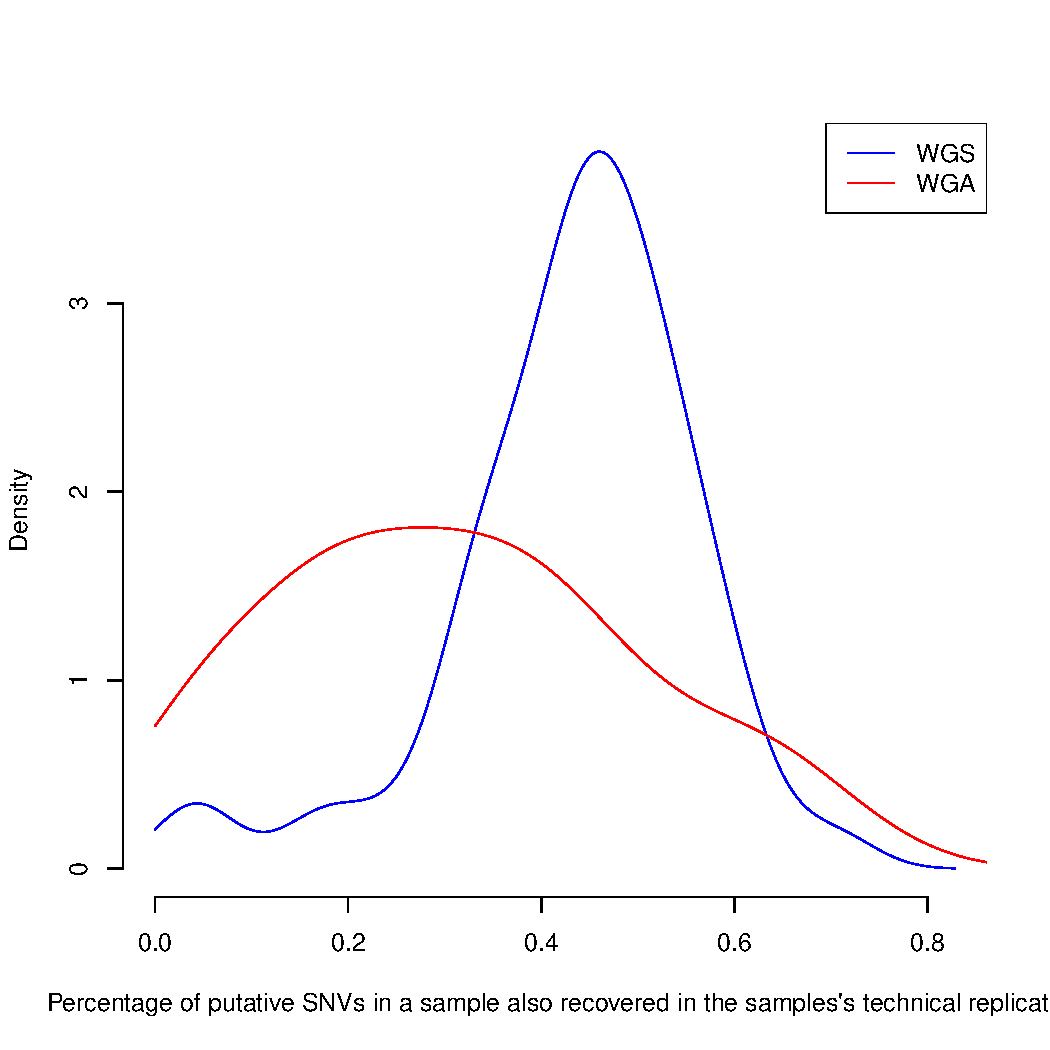
\includegraphics[width=5in]{orig_Figure3.pdf} }
\caption{\textbf{One third (WGA) to one half (WGS) of putative SNVs were recovered in technical replicates.} Density of the percentage of each WGS (blue) and WGA (red) sample that is present in the overlap between replicates for each patient. The WGS distribution is higher and narrower, showing that the WGS samples overall have a higher percentage overlap than the WGA samples, and less range in this parameter.}
\label{fig:density}
\end{figure}


\section{Tables}

%% Data processing commands table
\begin{landscape}
\begin{table}
\caption{\textbf{Back-end Processing.} This table shows the software packages we used in data processing, what we used each piece of software for, and the command associated with it. The rows are in order of use.}
\label{tab:commands}
\begin{tabular}{ p{2.5cm} p{6cm} p{12cm} }
	software & purpose & command\\
	\hline
	picard & regenerate fastq files from BAM file aligned to hg18 & \texttt{java -d64 -Xmx4g -jar SamToFastq.jar I=\$pfx.bam F=\$pfx.1.fastq F2=\$pfx.2.fastq 2$>$\&1} \\
	bwa & align fastq files to hg19 & \texttt{bwa aln -q 30 -t 8 \$hgReference \$fastq $>$ \$fastq.aln.sai} \\
	bwa, samtools & convert aligned fastq files into new BAM file & \texttt{bwa sampe -a 600 -P -r "\$RG" \$hgReference \$fastq1.aln.sai \$fastq2.aln.sai \$fastq1 \$fastq2 | samtools view -bSh -o \$outprefix.bam -} \\
	samtools & sort and index new BAM file & \texttt{samtools sort -@ 16 \$outprefix.bam \$outprefix.sorted 2, samtools index \$outprefix.sorted.bam 2} \\
	samtools & remove duplicate reads from BAM files & \texttt{samtools rmdup ../\$tumorpfx/\$tumorpfx.out.sorted.bam \$tumorpfx.dedup.bam} \\
	GATK & indel realignment & \texttt{java -d64 -jar \$gatkJar -R \$hgReference -T IndelRealigner -rf BadCigar -I \$tumorpfx.dedup.bam -known \$G1000.Mills -known \$G1000.Phase1.Indels -targetIntervals \$tumorpfx.intervals -o \$tumorpfx.realn.bam} \\
	GATK & base recalibration & \texttt{java -d64 -jar \$gatkJar -nct 8 -T BaseRecalibrator -rf BadCigar -I \$tumorpfx.realn.bam -R \$hgReference -knownSites \$dbSNP -o \$tumorpfx.recal.grp} \\
	samtools & index recalibrated BAM file & \texttt{samtools index \$tumorpfx.realn.recal.bam} \\
	SomaticSniper & call somatic mutations, generate VCF & \texttt{bam-somaticsniper -q 40 -Q 40 -J -s 0.001 -F vcf -f \$hgReference \$tumorbam \$normalbam \$tumorpfx.SS.vcf} \\
\end{tabular}
\end{table}
\end{landscape}

\end{document}
